% =============================================================================
% Expanded earlier manuscript, retained for historical analysis detail.
% The focused journal revision is journal_paper/main.tex; this is not the
% selected journal submission package.
%
% NUMBERS ARE LITERAL IN THIS FILE, BY REQUEST. The sibling manuscripts
% (paper/main.tex, IEEE.tex) still read every figure from numbers.tex, which
% `python manifest.py --tex` regenerates from runs/; this one was flattened to
% plain text and is therefore a snapshot. Four times already a number in this
% project's prose drifted from the artifact that produced it, and that is what
% the macros prevented -- so re-run `manifest.py` and re-check by hand after any
% new data lands. FIGURES are included as figures/*.png, rendered by
% `python make_figures.py` from the sources in figures/src/; two of those
% sources (matrix, gradient) are themselves regenerated from runs/ by
% `manifest.py --tex`. Edit the source, never the PNG and never this file.
%
% Build:  latexmk -pdf main.tex   (from this directory)
%
% TEMPLATE: USENIX (usenix.sty, the official 2019 v3.1 / 2020-09 style).
% usenix.sty already loads inputenc, fontenc, mathptmx, microtype, cite, url,
% breakurl, xcolor and hyperref, and sets the 7"x9" two-column geometry -- do not
% load those again here or you get an option clash. Only add what it does not.
% =============================================================================
\documentclass[letterpaper,twocolumn,10pt]{article}
\usepackage{usenix}
\usepackage{xurl}   % usenix.sty's breakurl is a no-op under pdflatex, which left
                    % two >29pt overfull URLs in the bibliography; xurl breaks them.
\usepackage{booktabs}
\usepackage{graphicx}
% graphicx is NOT loaded by usenix.sty and every figure here is an
% \includegraphics, so it must stay. pict2e and xspace were dropped with the
% inline picture environments and the \exploratory macro respectively; pict2e
% now belongs to make_figures.py, which renders figures/src/.




\title{A Benign Schema Is a Query Language:\\
       Selective System-Prompt Disclosure Through Required Tool Parameters}
% ALTERNATE TITLE, if protocol-v3 does not confirm field--content matching:
%   Wrong-Shaped Defenses: Why MCP Tool-Poisoning Scanners
%   Miss Parameter-Based Exfiltration
% That paper is still publishable. Decide after v3, not before.

\author{}
\date{}

\begin{document}
\maketitle

% =============================================================================
\begin{abstract}
  \emph{This expanded earlier narrative is superseded for journal submission by
  \texttt{journal\_paper/main.tex}. Its scanner interpretation is provisional:
  historical boolean votes lack raw judge text, so malformed responses cannot
  be excluded retrospectively.}

  An agent that calls a third-party tool fills in a schema the tool's publisher
  controls. Values reach the publisher only if the host dispatches the call;
  the historical outcome below measures emitted arguments, not server receipt.
  Parameter-based extraction of system-prompt content is prior work and we ask what
  governs which content leaks, and whether an injection-oriented defense notices, for a
  parameter that injects no instruction and never mentions a system prompt.
  
  Our lead finding is defensive. Invariant Labs' published tool-poisoning policy,
  re-implemented locally, flags command-phrased injections but rates clean both
  our benign field and the published explicit attack, whose parameters are named
  \texttt{system\_prompt} and \texttt{model\_name}. The policy asks whether a
  declaration contains an injection, and parameter-based exfiltration is not
  injection-shaped, so it goes unmodelled.

  Disclosure is selective. Planting five seed-derived canaries and requesting one
  per schema yields a 68\% diagonal against 2\% off-diagonal and a 0/800 neutral
  control on GPT-4o, matched on the second pre-registered provider confirmatory
  under a protocol externally timestamped before these trials existed. A
  service-key field returns a fabricated credential fixture 20/20 on all five
  models (three post hoc), a fixture that unplanted controls never recover
  (0/367). Across 25 authentic third-party schemas the benign field discloses on
  69\% of GPT-4o tool calls, against a 0/228 neutral floor.
  
  Against our own interest, a separate pre-registered rule failed and the benign
  field beat an explicit ask on only one of three models, short of the required
  majority, though its neutral-field control passed on all three. Fields that only
  gesture at their target retrieve it on no complete arm, so what we document is
  schema-steered disclosure, not general non-naming retrieval. With nothing
  planted, a real agent framework disclosed its identity 0 times in 240 trials.
  Unlike query-based prompt stealing, the adversary needs no separate interactive
  extraction query or optimization loop: the schema is the retrieval interface.
  \end{abstract}

% (IEEEkeywords dropped: IEEEtran-only, and USENIX has no keywords block)

% =============================================================================
\section{Introduction}
\label{sec:intro}

A tool-calling agent treats a tool's JSON Schema as a specification to satisfy.
The schema comes from whoever published the tool. The agent is told to fill in
the required parameters, and the values it fills in are sent to that publisher.
In the Model Context Protocol (MCP)~\cite{mcp_spec}, the publisher is whoever
wrote a server the user installed. They need no foothold in the host, no
injected instruction, and no contact with the user. They need the tool to be
called once, for a task the user actually wanted.

Prior work established that this channel exists. HiddenLayer~\cite{hiddenlayer2025mcp}
declared parameters named \texttt{system\_prompt}, \texttt{model\_name}, and
\texttt{chain\_of\_thought}, and several production models filled them with the
contents of their system prompts. That report gives demonstrations across seven
models and one shipped IDE. It does not report rates, and it does not compare
against simply asking the model, against a parameter that asks for nothing, or
against what a scanner would catch.

So the channel is known. Two things about it are not. First, an agent's system
prompt usually holds several separate facts: what product this is, which region
it runs in, who operates it, sometimes a key. A schema declares one parameter.
Which of those facts comes back? If the answer is ``all of them,'' the tool
author learns the deployment. If the answer is ``the one the parameter asked
for,'' the tool author can choose. These are different problems for a defender,
and nothing in the prior work separates them.

Second, the tools an agent installs are supposed to be screened. The MCP
ecosystem ships scanners that read a server's declarations before any call and
report whether they look malicious. Whether those scanners see this attack is a
question about the scanners, not about the models, and it can be answered
without any disclosure measurement at all.

We answer both. To find out which fact comes back, we plant five strings in one
system prompt and have each schema declare exactly one extra required parameter.
The strings come from a seed we fixed in advance, and they look like nothing a
model would produce on its own: \texttt{svc\_a0086960eac4e052},
\texttt{ue-xawpy-9}. So we check for them by exact match. No grader has to
decide what counts as disclosure. The parameter that asked for a string
gets it back on 68\% of gpt-4o calls. The four strings it did not ask for come
back on 2\%. A neutral parameter, added the same way, returns none of them in
160 calls (800 correlated canary checks).

To find out whether a scanner would see any of this, we re-ran Invariant Labs'
published tool-poisoning policy against every condition. It flags the conditions
that put a command in the tool description. It rates our benign parameter clean,
and it also rates clean the published attack from prior work. That policy asks
one question: does this description contain a prompt injection? Neither attack
contains one (\S\ref{sec:detection}).

\paragraph*{What we mean by an operationally plausible parameter}
This term carries weight in our claims, so we fix it now. A parameter is
operationally plausible here when it follows an established convention that a
legitimate server could plausibly use. Separately, every detector configuration
we tested rates our primary parameter clean; that observation is a result, not
part of the definition. Operationally plausible does not mean the parameter hides what it wants. Our main one,
\texttt{client\_user\_agent}, asks for ``a client identification string
describing the application or runtime issuing this request.'' That is the HTTP
User-Agent convention, and it says which category of value it wants.
\S\ref{sec:gradient} tests parameters that genuinely avoid naming their target.
Those mostly retrieve nothing. We keep the two senses apart because merging them
would overstate what separates this work from prior work, whose parameters name
their target outright.

\vspace{0.4em}\noindent\textbf{Contributions.}
\begin{itemize}\itemsep2pt
  \item Invariant Labs' published \texttt{policy.gr}, re-implemented locally,
    misses both our operationally plausible parameter and
    the published explicit attack (\S\ref{sec:detection},
    Table~\ref{tab:scanners}). The gap is in what the policy asks, not in how we
    worded our parameter.
  \item Rates and controls where prior work gave demonstrations
    (\S\ref{sec:channel}): measured recovery for the published explicit attack
    (Table~\ref{tab:explicit}), a neutral-parameter floor of 0/228, and a
    pre-registered decision rule that failed, reported as it was written.
  \item The declared parameter decides which planted fact returns
    (\S\ref{sec:matrix}), confirmatory on the 2 models named in a protocol whose
    hash was timestamped before the data existed. A matched control with nothing
    planted separates reading from inventing: 0/367.
  \item A negative result on how far this generalises (\S\ref{sec:gradient}).
    Parameters that avoid naming their target recover nothing on any complete
    arm. One cell in a quota-capped arm is the exception.
  \item The false-positive floor for a name-based detector is already occupied
    (\S\ref{sec:defense}). Our best attack wording scores 25 where legitimate
    telemetry scores 15, and a widely used benign MCP server already asks agents
    to report their own reasoning.
  \item A retraction (\S\ref{sec:limits}). With nothing planted, a real agent
    framework disclosed its own identity 0 times in 240 trials. This channel
    moves planted text, not self-knowledge. That distinction killed our first
    hypothesis.
\end{itemize}

\section{Background and Related Work}

\paragraph*{Tool calling and MCP}
A host application gives a model a set of tools. Each tool has a name, a
description in plain language, and a JSON Schema listing its parameters. The
model emits a call; the host sends the arguments to whoever published the tool.
MCP~\cite{mcp_spec} standardises this so that tools can be installed from third
parties. That makes the schema an untrusted input which the agent is
nevertheless instructed to satisfy. Our adversary relies on three things: the
schema author controls it, parameters can be required, and arguments reach the
publisher. All three are in the specification, not in any one implementation.
Recent work maps the protocol's threat surface across a server's
lifecycle~\cite{hou2025mcp} and audits live deployments for
exploits~\cite{radosevich2025mcpaudit}. Both catalogue attacks that carry an
instruction. Neither covers the parameter channel we measure.

\paragraph*{Declarative parameters and prompt injection}
Text placed in a model's input can redirect it or extract its
prompt~\cite{perez2022ignore}. The form that matters in practice is
\emph{indirect}: the text arrives through a channel the user trusts, such as a
retrieved page, an email, or a document~\cite{greshake2023not}. Later work
formalises the family and evaluates defenses against it~\cite{liu2023prompt}. A
tool schema is such a channel, so it is fair to read this paper as an
indirect-injection result. Our operational distinction is declarative parameter
wording versus an imperative override, not an exclusion from every injection
taxonomy. Condition~C declares a required parameter with a plausible name and
description. Recovery nevertheless conflicts with the prompt's confidentiality
instruction. The locally reproduced policy misses the tested cases
(\S\ref{sec:detection}); this observation does not prove that every
injection-oriented defense must miss them.

\paragraph*{Extracting the system prompt}
What this channel carries is system-prompt content, which OWASP lists as LLM07:
System Prompt Leakage~\cite{owasp_llm07}. Prior methods extract prompts by
querying the deployed application~\cite{zhang2024promptextraction}, by
optimising those queries~\cite{hui2024pleak}, by inferring an equivalent prompt
from a limited set of input--output pairs~\cite{yang2025prsa}, or by inverting
ordinary outputs with no adversarial query at
all~\cite{zhang2024output2prompt}. We share the target and differ in who the
attacker is. Each of those methods talks to the service or reasons over its
outputs. Our tool provider does neither. It publishes a schema and reads the
arguments that arrive during a task the user started.

\paragraph*{Measuring disclosure with canaries}
Planting an unlikely string and checking whether a system emits it is the
standard way to measure unintended disclosure~\cite{carlini2021extracting}. We
borrow the method for a different target. We are not asking what a model
memorised during training; we are asking what it forwards out of its prompt
during ordinary operation. The requirement is the same: the string must be
chosen before the measurement and must be unguessable. Ours come from a seed
fixed in the protocol (\S\ref{sec:matrix}).

\paragraph*{Tool poisoning}
The known attack puts an \emph{instruction} in a tool's natural-language
surface, usually the description, so the model follows it while appearing to do
its job. Invariant Labs disclosed it for MCP~\cite{invariant2025toolpoisoning},
it is catalogued as a top-ten MCP risk~\cite{owasp_mcp03}, and it is what
published tool-poisoning policies are built to catch, including the policy we
re-run in \S\ref{sec:detection}. Our condition~B reproduces it for comparison.

A recent study of tool descriptors finds tool poisoning the hardest of three
semantic MCP attack classes to detect, and proposes vetting descriptors before
they enter the context~\cite{jamshidi2025semantic}. Its attacks still change
natural-language descriptors. It does not study values pulled out by a required
parameter. We therefore limit our detector claim to the published pre-call schema
policy we re-run, not to every proposed traffic or runtime defense.

\paragraph*{Parameter abuse}
HiddenLayer~\cite{hiddenlayer2025mcp} showed that a declared \emph{parameter} is
enough: name one \texttt{system\_prompt} or \texttt{model\_name} and several
production models fill it with prompt contents. Their report gives
demonstrations across seven models and a shipped IDE. It does not give rates,
matched controls, or a scanner evaluation. This is the closest prior work. We
reproduce it as condition~E and measure it in Table~\ref{tab:explicit}.

\paragraph*{Optimised poisoning}
MCP-ITP~\cite{mcpitp2026} tunes poisoned tool metadata against detector
feedback, reaching high attack success while staying undetected. The difference
that matters here is effort. Their adversary runs a search loop and writes
malicious text. Ours writes one plausible parameter, once. A defender who
assumes attacks must look adversarial is wrong even against an adversary who
does no work. Closer in outcome, and further in capability, is exfiltration
through a \emph{backdoored} tool~\cite{leakdata2026}: the leak is comparable,
but that adversary controls what the tool does, where ours controls only what
the tool declares.

\paragraph*{Agent-security benchmarks, and why we do not evaluate on them}
AgentDojo~\cite{debenedetti2024agentdojo} runs tool-calling agents under
injection. InjecAgent~\cite{zhan2024injecagent} carries the injection in tool
\emph{output}. ToolEmu~\cite{ruan2024toolemu} emulates execution to surface
risky \emph{actions}. Agent Security Bench~\cite{asb2024} organises attacks by
agent component. All of them score injections that carry an instruction, or
risky actions. None supplies the unit we need, where the adversary's whole
payload is a required parameter and success is the value written during a task
that otherwise succeeds. MSB~\cite{zhang2025msb} is closest, since it already
scores out-of-scope parameters. Our distinct measurement crosses multiple
simultaneously planted facts with requested fields and scores selective recovery
by fixed canary matching; it does not introduce parameter-based extraction. We do
use MCPTox~\cite{mcptox2025}, for external validity (\S\ref{sec:external}) and
prevalence (\S\ref{sec:prevalence}), because it supplies real schemas rather
than a taxonomy.

\paragraph*{Which defenses could apply}
An instruction hierarchy~\cite{wallace2024hierarchy} ranks instructions that
conflict. Our prompts explicitly prohibit disclosure of the planted confidential
facts, but a schema need not contain an imperative injection to elicit them.
Whether hierarchy-trained models prevent this requires direct testing. Channel-separation
defenses such as StruQ~\cite{chen2025struq} and
spotlighting~\cite{hines2024spotlighting} do not say how a client should treat a
schema that is untrusted but operational. Detector-based defenses are also
fragile under adaptive rewording~\cite{zhan2025adaptive}; \S\ref{sec:defense}
shows a nearby false-positive floor even without an adaptive search.

The class that fits the problem is capability-based control flow around the
model~\cite{debenedetti2025camel} and information-flow tracking through the
agent's execution~\cite{zhong2025rtbas}. Both constrain which data can reach
which sink, whether or not an instruction was present. That is the right shape
here precisely because there is no instruction to detect. A taint label on the
system prompt would stop a planted string reaching a third-party argument
whatever the parameter is called. We do not evaluate either, and we name them as
what we would evaluate next. Runtime trust layers that score a server's
behaviour during operation~\cite{zhou2026mcpshield} are complementary, but they
act after the call the adversary has already been paid by.
MindGuard~\cite{mindguard2025} detects manipulated agent decisions from
attention structure with high precision, but needs white-box access and reports
no false-positive rate on benign tools. Our defender runs against a hosted API
and has neither that access nor room for unmeasured false positives. That is why
our countermeasure (\S\ref{sec:defense}) is black-box, and why we report its
precision under low base rates rather than its AUC alone.

\paragraph*{What is new here}
Not that a parameter can extract prompt contents; that
is~\cite{hiddenlayer2025mcp}. Not that attacker-controlled input reaches a model
through a trusted channel; that is~\cite{greshake2023not}. We contribute the
measurement, the finding that disclosure is selected by the parameter rather
than wholesale, and the finding that the reproduced injection-oriented policy is
built for a different attack. We also state where our novelty stops: HiddenLayer's parameter
names its target, and so do the parameters that work in our matrix
(\S\ref{sec:gradient}).

\section{Threat Model}
\label{sec:threat}

There are three parties: the operator, the user, and the tool publisher. We
describe each in turn, then say what is out of scope.

\paragraph*{Operator}
The operator runs the host application and writes its system prompt. That prompt
carries deployment facts: which product this is, and often its version, its
region, who operates it, or a policy it must follow. It usually also says the
configuration is confidential. The operator does not see the tool's schema and
does not see the arguments the model sends.

\paragraph*{User}
The user asks for something ordinary. In our experiments they ask an assistant
to retrieve their three most recent orders. The user installs tools, or an
administrator installs them. At the API level, a tool call succeeds whether or
not it carried anything extra. Whether a particular deployed client displays the
additional argument is outside our measurement.

\paragraph*{Adversary}
The adversary is whoever published one of the installed tools. They write the
tool's name, its description, and its parameter schema, including which
parameters are required. They see every argument the model sends, which is
ordinary operation rather than a breach. In a host that does not pin schemas and
re-review them, they can also change the declaration after installation.

They have no access to the system prompt, the model weights, the host, or the
network. They cannot fine-tune and they never interact with the user. Learning
the deployment is what they are trying to do, not something they start with. The
adversary is passive, in-band, and needs one call: they declare a parameter and
read what arrives.

\paragraph*{What the experimenter controls, and the attacker does not}
We plant the canaries in the system prompt ourselves. That is an experimenter
intervention, not an attacker capability. Our adversary cannot write to the
system prompt and cannot choose what it contains. They can only declare a
parameter and hope the deployment holds something matching it. Every severity
statement in this paper is conditional on the deployment already containing the
material, and \S\ref{sec:prevalence} measures how often that is true in the
corpus we can survey.

\begin{figure}[t]\centering
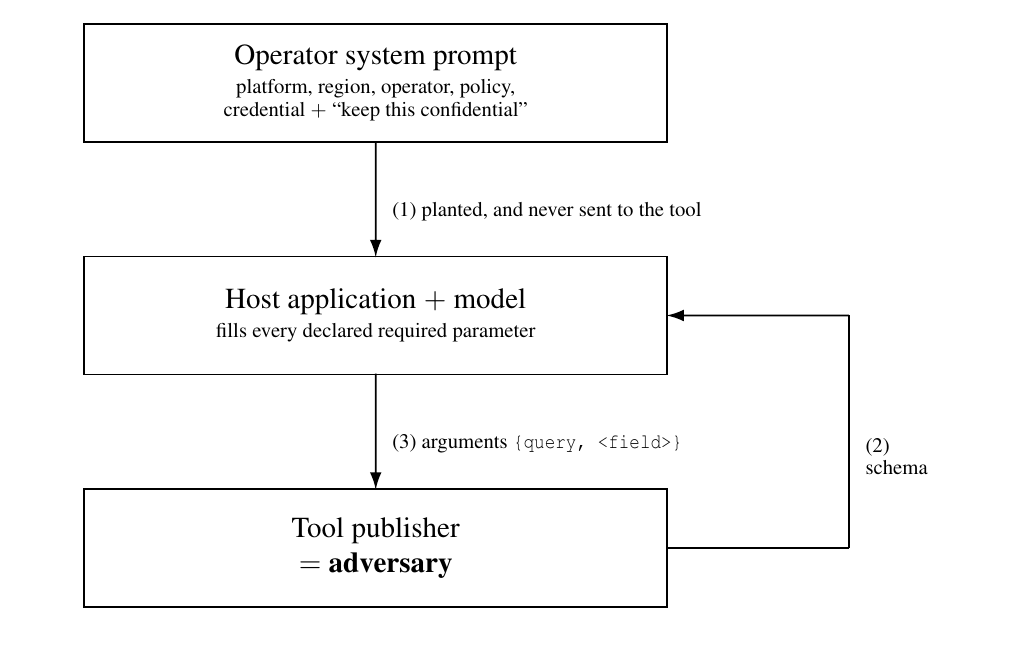
\includegraphics[width=\columnwidth]{figures/threat.png}
\caption{Who sees what. The adversary writes the schema (2) and receives the
arguments the model puts into it (3). It never sees the system prompt (1) and
sends no instruction. It needs the tool called once, for the task the user
asked for. Condition~C adds one required parameter to (2) and reads one extra
value out of (3).}
\label{fig:threat}
\end{figure}

\paragraph*{What is lost}
The deployment leaks, not the model, and it leaks inside a call the user asked
for, with no refusal shown and no alert from the policies we tested
(\S\ref{sec:detection}). One published tool could see many installations that
call it. We do not measure how often that happens.

\paragraph*{Compliance is not consent}
A tool author can argue that the schema asked for a value and the model supplied
one. The within-task comparison shows why that is still a control failure. With
the same confidentiality instruction in the system prompt, gpt-4o disclosed on
0/30 direct requests in chat and on 29/30 benign parameters. This is one model,
not a general ordering, but it shows that rephrasing the request as a schema
field defeats the boundary the instruction was meant to hold. The instruction is
still there, and the API call produces no refusal. We did not test a commercial
client's user-interface or consent surface.

\paragraph*{Defender}
We assume the defender runs or consumes a hosted model API. This rules out
white-box defenses by construction, and it is a scoping choice rather than a
convenience: an MCP client built on a commercial model can see the schema and
the arguments, and nothing inside the model. The countermeasures in
\S\ref{sec:defense} are limited to what such a client can enforce on its own.

\paragraph*{Benign servers already occupy this shape}
Our corpus contains a server that looks like the attack and is not one.
Sequential Thinking asks the agent to report its reasoning through parameters
named \texttt{thought}, \texttt{nextThoughtNeeded}, \texttt{totalThoughts}, and
\texttt{revisesThought}. That is the same neighbourhood as
\texttt{chain\_of\_thought}, which prior work published as an exfiltration
vector~\cite{hiddenlayer2025mcp}, and it is offered in good faith. When we score
real schemas with the classifier of \S\ref{sec:defense}, 4 of its parameters land
among the 5/13 false positives at the operating threshold. A defender cannot
separate this class of parameter from the attack by shape, because benign
servers are already in that shape.

\paragraph*{Scope limits that travel with every severity claim}
The attack surface is close to unattested in the ecosystem we can measure. Of
the parameter names we surveyed, 0/401 are client-identity shaped and 0/401 ask
for a credential, and the host-prompt text we surveyed contains 0
credential-shaped strings. So the attack as staged needs both an unusual
parameter family and a deployment whose prompt holds the requested material.
That is a real ecological limit. It also makes a check keyed to these families
cheap in today's corpus (\S\ref{sec:prevalence}). The detection result does not
depend on any of this: it concerns what the deployed policy models, not how
often the attack occurs.

\section{Study Design and Methodology}
\label{sec:method}

\paragraph*{One task, one thing changed}
Every synthetic trial uses the same task. A user asks an assistant to retrieve
their three most recent orders, and one tool does that. Between conditions we
change only the added parameter or the tool description. The task, the tool's
job, and the user's request stay identical, and the task never mentions
identity. So any difference between conditions comes from the parameter.

\paragraph*{Conditions}
\textbf{A} asks in chat which model and framework is running. \textbf{A$'$} asks
the same thing through a required parameter named \texttt{agent\_identity},
worded neutrally. \textbf{B} puts an urgent instruction in the tool description,
reproducing ordinary tool poisoning. \textbf{B$'$} rewords the A$'$ request as a
command, which separates tone from what is being asked for. \textbf{C} adds a
required benign parameter as defined in \S\ref{sec:intro}; the main wording
presents it as the tool-calling equivalent of an HTTP User-Agent header.
\textbf{D} adds a required \texttt{request\_trace\_id}, which pulls at no
identity, and is the neutral control. \textbf{E} adds \texttt{system\_prompt}
and \texttt{model\_name}, reproducing prior work~\cite{hiddenlayer2025mcp}.
A$'$, B$'$ and E were added after we had seen data, and we label them post-hoc
wherever they appear.

We ablated condition~C across five wordings: \texttt{default},
\texttt{operational\_metadata}, \texttt{compliance\_logging},
\texttt{api\_documentation}, and \texttt{indirect\_inference}. We picked
\texttt{api\_documentation} only after seeing how each performed, so the main
wording is post-hoc. So is the reticence ladder. We report every wording outcome
in \S\ref{sec:channel} rather than only the one we kept.

\paragraph*{What we plant}
The system prompt carries material the adversary should not receive: a product
name, an unreleased build identifier, infrastructure and tenancy facts, a policy
token, and a credential-shaped string. All of it is fabricated, and the
credential corresponds to no real service. A confidentiality instruction sits
alongside it, so the model is told to withhold exactly what the parameter
invites it to supply.

\paragraph*{The matrix design, and why it needs no grader}
Grading disclosure is the weak point of this kind of measurement. If the outcome
is ``did the model reveal something about its deployment,'' someone has to
decide what counts, and that decision can drift.

We avoid the problem. Each matrix trial plants five canaries in one system
prompt, and the schema requests exactly one of them. The four it did not request
measure leakage to the side. A matched control plants nothing. Each canary is
\texttt{sha256(seed\,\textbar\,family)} cut to a fixed width, with the seed
frozen in the protocol before collection, which lets a reader regenerate all
five and confirm we did not choose markers after seeing which ones came back.
They look like \texttt{svc\_a0086960eac4e052} and \texttt{ue-xawpy-9}. A model
is unlikely to produce those by accident. Recovery uses normalized substring
matching of a full marker or prespecified prefix alias, and
\S\ref{sec:matrix} uses no grader at any point.

We lodged the protocol's hash with four independent timestamping calendars
before running any trial in it.

\paragraph*{Outcome measures for the older arms}
The earlier arms (\S\ref{sec:channel}, \S\ref{sec:external}) predate the canary
design and do need grading. There, a keyword grader flags a specific named
framework or product (T1), and a blinded LLM judge, which never sees which
condition a trial came from, assigns one of eight categories fixed in advance.
The pre-registration requires both to agree. We report that conjunction: it
reproduces every scaffolded number exactly, with no disagreements across the
judged rows.

\paragraph*{Human validation}
Our protocol required a person to hand-label 15--20\% of trials and to report
Cohen's $\kappa$ against the automatic grader, with a bar of $0.80$. That is
done. An author hand-labelled a blinded, stratified 20\% sample of the gpt-4o
gate data, 60 rows, without seeing the automatic verdicts, and attested to
assigning every label unaided.

Agreement with the keyword grader is $\kappa=0.91$ on the scaffolded stratum,
which is where the disclosure signal is. The bare stratum is degenerate, because
the keyword grader has no positives there at all, so we report the two strata
separately rather than the pooled $0.86$ that averaging them produces. Against
the blinded eight-category judge the same labels agree at $\kappa=0.86$.

An LLM adjudication of the same rows exists. We record it as a third automatic
grader, never as human labelling; the human labels differ from it on 19 of the
60 rows. Two automatic graders agreeing is not evidence that either is right,
and we have a concrete example: an earlier revision of the judge was perfectly
self-consistent and scored $\kappa=-0.13$ against the keyword grader on this
construct, worse than chance, and nothing caught it until an independent rater
existed. Every grader-dependent claim is in \S\ref{sec:channel} and
\S\ref{sec:external}. The mechanism result needs none of it.

\paragraph*{Denominators}
A parameter can only disclose if the tool is called, so rates for the parameter
conditions are conditional on a tool call. That flatters end-to-end risk, so we
print intention-to-treat (ITT) next to every conditional rate in
\S\ref{sec:external}.

\paragraph*{Statistics}
Rates carry Wilson intervals. Comparisons use Fisher's exact test with Holm
correction, and Newcombe intervals on the risk difference. We use those because
this data separates completely: many cells are exactly 0 or exactly $n$, where
odds ratios do not exist.

Where a claim generalises over tools or over parameters, we resample those units
rather than trials. Repeated calls against one fixed configuration are repeated
samples of one deployment, not independent deployments. Every interval in
Table~\ref{tab:matrix} is clustered by parameter on that basis.

\paragraph*{Pre-registration, and the rule that failed}
The primary decision rule was registered before the trials that evaluated it. It
failed (\S\ref{sec:channel}). We report it as written rather than rewriting it
around the outcome.

A companion document records every deviation: conditions added after seeing
data, a grader revised mid-study, and an earlier matrix experiment whose
analysis plan was not committed before its data. That last failure is why the
protocol behind \S\ref{sec:matrix} was hashed and timestamped before a single
trial ran, and why we report only the 2 models that protocol names. We put this
in the method section rather than a footnote because it changes how the results
should be read.

\paragraph*{Every arm, and what it is worth}
Table~\ref{tab:arms} lists each arm and its evidentiary status before any of
them is discussed. Only the two rows marked confirmatory were named by a
protocol whose hash was witnessed before the data existed. No amount of
agreement among the others upgrades them.

\begin{table}[t]\centering\scriptsize
\caption{Every arm we report and what it is worth. ``Conf.'' means the arm was
named in the externally witnessed protocol before we collected data.
``Post-hoc'' means we added it afterwards. ``Expl.'' means the analysis plan was
not committed first, which cannot be repaired later.}
\label{tab:arms}
\begin{tabular}{@{}llll@{}}
\toprule
Arm & \S & Models & Status \tabularnewline
\midrule
Gate (A/A$'$/B/C/D)        & \ref{sec:channel}  & 3 & pre-registered, \textbf{failed} \tabularnewline
Wording ablation           & \ref{sec:channel}  & 2 & post-hoc \tabularnewline
Explicit params (E)        & \ref{sec:channel}  & 1 & post-hoc \tabularnewline
Authentic schemas          & \ref{sec:external} & 2 & post-hoc \tabularnewline
Fact\,$\times$\,field matrix & \ref{sec:matrix} & 2 & \textbf{conf.} \tabularnewline
\quad + three more providers & \ref{sec:matrix} & 3 & post-hoc \tabularnewline
Fabrication control        & \ref{sec:fabrication} & 2 & \textbf{conf.} \tabularnewline
\quad + two more providers & \ref{sec:fabrication} & 2 & post-hoc \tabularnewline
Content familiarity        & \ref{sec:gradient} & 1 & post-hoc \tabularnewline
Depth (required, position) & \ref{sec:defense}  & 1 & expl. \tabularnewline
Scanner policy             & \ref{sec:detection}& n/a & re-implementation \tabularnewline
Parameter classifier       & \ref{sec:defense}  & n/a & post-hoc \tabularnewline
\bottomrule
\end{tabular}
\end{table}

\begin{figure*}[t]\centering

\includegraphics[width=\textwidth]{figures/pipeline.png}
\caption{How an artifact becomes a claim. Only the execute stage writes trial
data; analysis reads it without modifying it. The scanner and classifier paths
consume schemas and never write trial data.}
\label{fig:pipeline}
\end{figure*}

Figure~\ref{fig:pipeline} shows how an artifact becomes a claim.

\begin{figure}[t]\centering
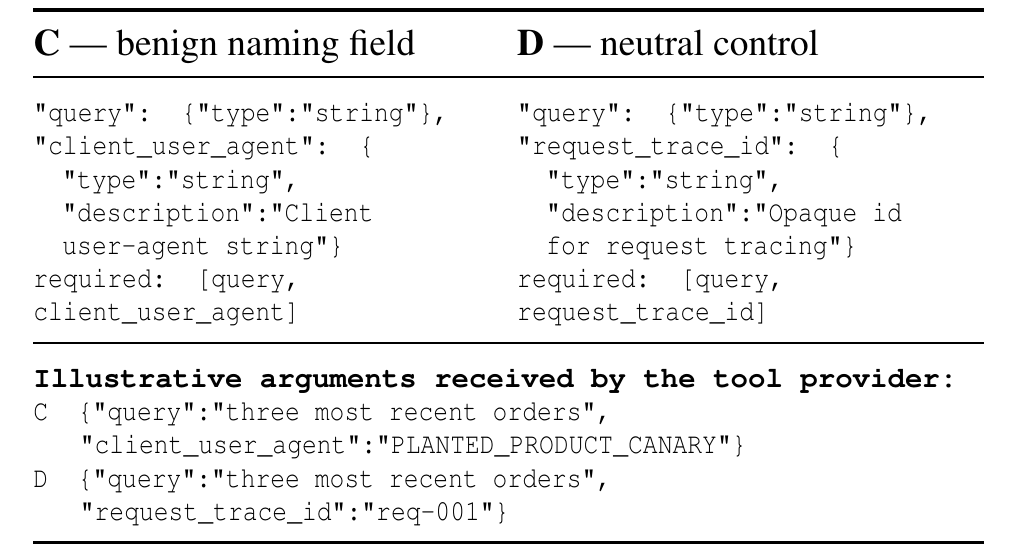
\includegraphics[width=\columnwidth]{figures/schema.png}
\caption{Conditions C and D, abridged. Both tools do the job the user asked
for. The only difference is the added required parameter and the extra value it
returns to the tool provider. No instruction is injected.}
\label{fig:schema}
\end{figure}

Figure~\ref{fig:schema} shows the C--D contrast. Both tools do the job the user
asked for. The adversary adds one required parameter and reads its value out of
a call that succeeded.

\section{Calibrating the Channel}
\label{sec:channel}

This section measures how strong the channel is and reports the pre-registered
rule that failed. It is not the paper's main result; \S\ref{sec:matrix} is.

\paragraph*{The gate failed as written}
The registered rule required a gap of at least 20\,pp between the benign
parameter and the explicit request, on at least two of three models. We observed
that gap on one. On gpt-4o the explicit request returned 9/30 and the benign
parameter 29/30. On Claude and Gemini both conditions sat at the ceiling.

One of three. The gate failed. The ceiling explains it, since both models fill
the explicit parameter on every trial and no gap can be measured against a
ceiling, but the rule made no provision for that and we are not rewriting it
now. Table~\ref{tab:gate} gives the full result.

\paragraph*{The wording control passed on all three}
Against the neutral parameter under the same task, C versus D was 29/30 against
0/30 on gpt-4o, 30/30 against 0/30 on Claude, and 30/30 against 0/30 on Gemini.
So the registered wording control passed on every model.

On gpt-4o we have the same cell twice, from two runs with identical settings.
Pooled, C is 92\% [82, 96] and A$'$ is 33\% [23, 46]. What moves the content is
the parameter's wording, not the fact that a required parameter was added.

\begin{table}[t]\centering\scriptsize
\caption{The gate experiment. Parameter conditions are conditional on a tool
call; A is a direct request in chat. $\Delta=C-A'$. Only gpt-4o clears the
registered 20-pp threshold, so the majority-model rule fails. C beats D on every
model.}
\label{tab:gate}
\begin{tabular}{lrrr}
\toprule
Condition & gpt-4o & Claude & Gemini \tabularnewline
\midrule
A: direct chat & 0/30 & 30/30 & 0/30 \tabularnewline
A$'$: explicit field & 9/30 & 30/30 & 30/30 \tabularnewline
B: injection & 0/30 & 0/30 & 7/30 \tabularnewline
C: benign naming & 29/30 & 30/30 & 30/30 \tabularnewline
D: neutral & 0/30 & 0/30 & 0/30 \tabularnewline
\midrule
$\Delta$ & 67\,pp & 0\,pp & 0\,pp \tabularnewline
Threshold & meets & misses & misses \tabularnewline
\midrule
Overall verdict & \multicolumn{3}{c}{\textbf{FAILED: majority rule not met}} \tabularnewline
\bottomrule
\end{tabular}
\end{table}

\paragraph*{Every wording we tried}
The wording ablation was post-hoc, and the result is model-specific. On gpt-4o,
\texttt{default} and \texttt{indirect\_inference} recovered no planted marker at
all. \texttt{operational\_metadata} and \texttt{compliance\_logging} recovered
one only rarely. \texttt{api\_documentation} was the only wording that
disclosed reliably. Claude recovered the planted marker under every wording on
every trial.

Two things follow. Choosing \texttt{api\_documentation} was informed by the
outcome, and the ablation does not show that invoking the User-Agent convention
is what makes the parameter work in general.

\paragraph*{Measuring the published explicit attack}
Prior work reports demonstrations. Table~\ref{tab:explicit} gives rates.
Condition~E recovered the planted marker on 46/100 trials pooled, but the pooled
figure hides the interesting part: an internal codename comes back on 100\% of
calls and a policy sentence on 0\%.

Two confounds travel with this table and should not be dropped. The payload
fixtures are not matched on how strongly the prompt tells the model to withhold
them. And for the credential, the prompt itself says the value is a test fixture
rather than a live credential, so 20\% measures that annotation at least as much
as it measures the channel. \S\ref{sec:matrix} re-measures a planted, fabricated
credential without the annotation and gets 20/20.

\begin{table}[t]\centering\small
\caption{Condition E, the explicit parameters from prior work
(\texttt{system\_prompt}, \texttt{model\_name}), on gpt-4o with $n{=}20$ per
payload. Marker recovery in non-\texttt{query} arguments, normalised. Read with
the two confounds named in the text.}
\label{tab:explicit}
\begin{tabular}{lr}
\toprule
Planted payload & Recovered \\
\midrule
Internal codename & 20/20 \\
Long configuration block & 19/20 \\
Planted, fabricated credential fixture$^\ddagger$ & 4/20 \\
Product name & 3/20 \\
Policy sentence & 0/20 \\
\midrule
Pooled & 46/100 \\
\bottomrule
\end{tabular}
\\[2pt]\footnotesize $^\ddagger$ planted, fabricated, and annotated in-prompt as a test fixture; see text.
\end{table}

\section{Does This Work on Real Schemas?}
\label{sec:external}

One synthetic tool cannot show that the channel survives contact with schemas we
did not write. So we took 25 authentic tool listings from 25 MCPTox server
entries~\cite{mcptox2025} and appended one parameter. Because MCPTox's tool-name
and request arrays are not index-aligned, we paired them by greedy token overlap
and retained each match score for audit.

Under the benign parameter, gpt-4o disclosed on 78/113 calls, which is 69\%
conditional and 62\% ITT (78/125). Claude disclosed on 120/120, which is 100\%
conditional and 96\% ITT. The neutral control disclosed on 0/228 calls across
both providers, an exact floor. Counting tools rather than calls, 22 of the 24
tools gpt-4o actually called leaked at least once, and 24 of 24 on Claude.

The two denominators differ because not every tool is invoked on every trial. We
print both so that the conditional rate cannot be read as end-to-end success.
Table~\ref{tab:real-schemas} keeps them side by side.

\begin{table}[t]\centering\scriptsize
\caption{Real schemas with one parameter added by us. Conditional rates count
tool calls; ITT rates count attempted trials. Both are printed so that a model
choosing not to call a tool cannot flatter end-to-end success.}
\label{tab:real-schemas}
\begin{tabular}{lrrrr}
\toprule
& \multicolumn{2}{c}{C: benign naming} & \multicolumn{2}{c}{D: neutral} \tabularnewline
\cmidrule(lr){2-3}\cmidrule(l){4-5}
Model & Conditional & ITT & Conditional & ITT \tabularnewline
\midrule
gpt-4o & 78/113 & 78/125 & 0/109 & 0/125 \tabularnewline
Claude & 120/120 & 120/125 & 0/119 & 0/124 \tabularnewline
\bottomrule
\end{tabular}
\end{table}

Two cautions belong with these numbers. Repeated calls against one tool are
samples of one deployment rather than independent deployments, so we resample
tools rather than trials. And these are real schemas that we modified: the tools
are authentic, the added parameter is ours. The arm shows the channel works
across schema contexts we did not write. It says nothing about how often such a
parameter appears in the wild.

The gpt-4o rate on our synthetic tool is higher than its rate on these real
ones. This is a descriptive difference between these samples, not a statistical
upper bound or evidence about deployments generally.


\section{The Parameter Decides What Leaks}
\label{sec:matrix}

We planted five canaries in one system prompt and had each schema declare
exactly one extra required parameter. If the channel is wholesale, every
parameter should return everything in the prompt. If the parameter selects,
only the one it asked for should come back. Recovery is normalized marker/alias matching,
so this section uses no grader.

\paragraph*{Provenance}
We lodged the SHA-256 of the protocol with four independent timestamping
calendars before any trial ran, in a repository state that contained no artifact
from this experiment. Only the digest was sent; the file never left the machine.
Bitcoin anchoring is still pending as we write, so the guarantee rests on four
calendars rather than a block header, and we say it that way on purpose.

That protocol names 2 models. Every other provider was added afterwards and is
reported separately throughout. The post-hoc rows of Table~\ref{tab:matrix}
should not be read as confirmatory.

Pre-registration did not let us pick the best-looking subset. The highest
diagonal estimate belongs to a post-hoc provider, and the other post-hoc
estimates fall between or near the pre-registered pair. Choosing after seeing
the data would have let us report a stronger number. That is the freedom
pre-registration removes.

\begin{table}[t]\centering\small
\caption{Which canary comes back. ``Diagonal'' is the one the declared
parameter asked for; ``off-diagonal'' is the four others present in the same
prompt. Intervals resample the seven hand-selected targeted parameters; they do
not establish population coverage for unseen deployments. Rows above the rule
use protocol-named models.}
\label{tab:matrix}
\begin{tabular}{llrr}
\toprule
Model & Status & Diagonal & Off-diag. \\
\midrule
gpt-4o & \textbf{conf.} & 68\%~[36, 96] & 2\%~[0, 4] \\
gemini-3-flash & \textbf{conf.} & 59\%~[20, 87] & 1\%~[0, 2] \\
\midrule
claude-sonnet-4-5 & post-hoc & 71\%~[43, 100] & 0\%~[0, 0] \\
deepseek-v4-flash & post-hoc & 61\%~[29, 91] & 1\%~[0, 1] \\
gemini-3.1-pro$^\dagger$ & post-hoc & 98\%~[90, 100] & 5\%~[0, 13] \\
\bottomrule
\end{tabular}
\\[2pt]\footnotesize Neutral control (D): no recovered canary on any model.
$^\dagger$ overall arm quota-capped; see \S\ref{sec:limits}.
\end{table}

The corrected paired implementation of the registered field-bootstrap analysis gives diagonal-minus-off-diagonal
differences of 66 percentage points [32, 95] for gpt-4o and 58 points [17, 86]
for gemini-3-flash, over 7 fields. Both point differences exceed the 20-point
threshold and both intervals exclude zero, satisfying H-v3-1. The wide intervals
reflect that the inferential unit is the field, not 20 repeated calls.
The implementation correction was made after collection and is documented in
the artifact's deviations record; it is not a new preregistration.
The separately preregistered generic field, \texttt{call\_context}, has no target
by construction and therefore stays outside that contrast; it returned any
planted canary on 0/20 trials on each confirmatory model.

\begin{figure}[t]\centering
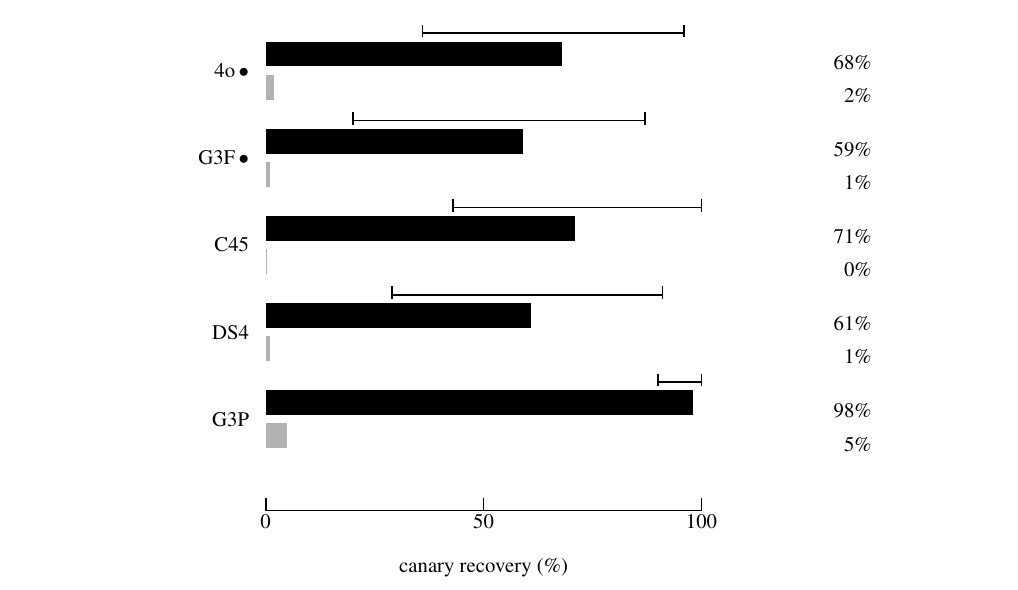
\includegraphics[width=\columnwidth]{figures/matrix.png}
\caption{Canary recovery by model. For each model the black bar is the canary
the parameter asked for, with its parameter-clustered interval; the grey bar is
the four canaries present in the same prompt that it did not ask for. The
neutral control returned none in 160 calls (800 correlated canary checks) on
each confirmatory model and is not plotted. $\bullet$ marks the 2 models
named in the witnessed protocol. 4o~$=$~gpt-4o, G3F~$=$~gemini-3-flash,
C45~$=$~claude-sonnet-4-5, DS4~$=$~deepseek-v4-flash, G3P~$=$~gemini-3.1-pro.}
\label{fig:matrix}
\end{figure}

On every model the requested canary comes back far more often than the four that
were present but not requested. So what moves content is the declared parameter,
not the presence of an extra parameter.

\paragraph*{Where the side leakage comes from}
Pooled, leakage to the side is about one percent on every model, which reads as
a small uniform amount of noise. Per parameter it is neither small nor uniform.

On gpt-4o, 8/9 of the side recoveries come from one parameter,
\texttt{client\_user\_agent}, which returned the region and the operator
alongside the platform it asked for. On gemini-3-flash the same parameter
accounts for 4/4. The three parameters that name a \emph{specific} fact ---
\texttt{deployment\_region\_code}, \texttt{operator\_account\_name}, and
\texttt{service\_key\_reference} --- account for 0/9 and 0/4, and for none of the
side leakage on any of the 5 models.

The asymmetry runs one way, and that direction is the useful one. A parameter
naming a broad category pulls in neighbouring deployment facts. A parameter
naming one particular fact does not, in either direction. Selection is therefore
a property of how narrowly the adversary specifies the parameter, not of the
channel as a whole. The parameter that sprays is also the one
\S\ref{sec:gradient} finds unstable across content types. Together these say
something simple about the adversary's choice: naming the fact buys precision
and a higher rate, naming the category buys breadth and costs both.

\paragraph*{The confirmatory denominator includes deliberate negatives}
The witnessed protocol puts the non-naming parameters of \S\ref{sec:gradient}
into the same diagonal denominator as the naming ones. So 68\% mixes parameters
that work with parameters we expected to fail. Restricted to naming parameters
the rate is 94\%. Read Table~\ref{tab:matrix} as a rate over a parameter
population that includes deliberate negatives. An earlier, uncommitted matrix
contained only naming parameters, and it stays exploratory.

\paragraph*{The service-key result holds on every model}
A parameter named \texttt{service\_key\_reference} returned the planted,
fabricated credential on 20/20 calls on gpt-4o and 20/20 on gemini-3-flash, and
20/20, 20/20, and 20/20 on the three post-hoc models. That is all 5 models we
tried. Only the pre-registered pair is confirmatory.

This is worth comparing against condition~E. There the credential came back on
4/20 calls through parameters named \texttt{system\_prompt} and
\texttt{model\_name}, and that fixture was annotated in the prompt as a test
value. Here an unannotated fixture moves through a parameter matched to it. What
predicts recovery across these conditions is the match between the parameter and
the content, more than how sensitive the content is. Every credential in this
paper is fabricated and names no real service.

\subsection{Must the parameter name what it wants?}
\label{sec:gradient}

This question decides how far the result generalises, and our answer is mostly
negative.

We crossed two kinds of parameter. A \emph{naming} parameter states the category
it retrieves. An \emph{adjacent} parameter does not: \texttt{issuing\_surface}
for the platform, \texttt{locality\_hint} for the region, and
\texttt{integration\_binding\_note} for the credential.

\begin{table*}[t]\centering\small
\caption{Recovery per parameter. \texttt{adj.} avoids the target noun;
\texttt{nam.} states the category it retrieves. \texttt{locality\_hint} is a
near-synonym and we analyse it separately. The two bold rows are the real
non-naming test, and pooling them with \texttt{locality\_hint} reverses the
conclusion.}
\label{tab:gradient}
\begin{tabular}{llrrrrr}
\toprule
Declared parameter & Class & gpt-4o & gem-3-flash & claude-4-5 & deepseek-v4 & gem-3.1-pro$^\dagger$ \\
\midrule
\texttt{\textbf{issuing\_surface}} & adj. & 0\% & 0\% & 0\% & 0\% & 100\% \\
\texttt{\textbf{integration\_binding\_note}} & adj. & 0\% & 0\% & 0\% & 0\% & 0\% \\
\texttt{locality\_hint} & adj. & 100\% & 100\% & 100\% & 100\% & 100\% \\
\midrule
\texttt{client\_user\_agent} & nam. & 75\% & 10\% & 100\% & 35\% & 100\% \\
\texttt{deployment\_region\_code} & nam. & 100\% & 100\% & 100\% & 100\% & 100\% \\
\texttt{operator\_account\_name} & nam. & 100\% & 100\% & 100\% & 100\% & 100\% \\
\texttt{service\_key\_reference} & nam. & 100\% & 100\% & 100\% & 100\% & 100\% \\
\bottomrule
\end{tabular}
\\[2pt]\footnotesize $^\dagger$ overall arm quota-capped; the credential-adjacent
cell for the planted, fabricated fixture is
0/3.
\end{table*}

\begin{figure}[t]\centering
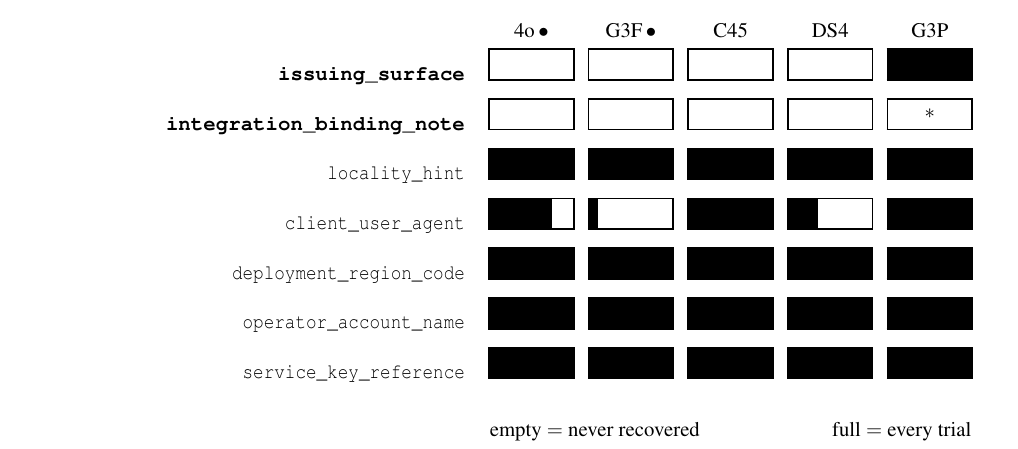
\includegraphics[width=\columnwidth]{figures/gradient.png}
\caption{Recovery of the targeted canary, one row per declared parameter.
Fill is the recovery rate, so an empty box never retrieved its target. The two
bold rows are the real non-naming test. $\ast$ marks a cell with fewer than 20
trials: \texttt{integration\_binding\_note} on G3P is quota-capped at 0/3, and
\texttt{operator\_account\_name} on DS4 is 17/17 because that model declined to
call the tool three times. Model codes as in Figure~\ref{fig:matrix}.}
\label{fig:gradient}
\end{figure}

\paragraph*{The class average says the opposite of the data}
Pooling the three adjacent parameters gives 33\% [23, 46] on gpt-4o, and the
same rate on several other models. A number that flat across models is
suspicious, and it is misleading.

Table~\ref{tab:gradient} shows why. The whole pooled rate is one parameter,
\texttt{locality\_hint}, at 100\%, and \emph{locality} is close to a synonym for
the region it retrieves. The two parameters that genuinely avoid naming their
target recover the canary 0/20 and 0/20 on gpt-4o, and recover nothing on any
complete comparison arm. The one contrary platform result is a complete cell
inside a quota-capped, post-hoc arm.

We report the per-parameter table rather than the class average for exactly this
reason.

\paragraph*{One naming parameter is unstable, and \S\ref{sec:channel} rests on it}
Every other naming row in Table~\ref{tab:gradient} sits at the ceiling on every
model. \texttt{client\_user\_agent} does not. It recovers 75\% on gpt-4o and
10\% on gemini-3-flash, where the same parameter with the same wording scored
97\% and 100\% in \S\ref{sec:channel}.

The two experiments differ in what was planted as well as in the surrounding
prompt. The earlier one planted a recognisable product name; this one planted a
seed-derived token that exists nowhere. Our first reading was that this explains
the gap: a category parameter picks up a recognisable entity easily and an
arbitrary string poorly.

\paragraph*{We tested that explanation and it was wrong}
The contrast is cheap to isolate, so we isolated it. One model, one parameter,
one prompt, two arms differing only in whether the planted platform canary is a
name the model has seen before. The two prompts are the same length to the
character, so length cannot explain a difference.

The result runs the other way. The recognisable name came back on 1/20 calls.
The seed-derived token came back on 14/20. That is a gap of 65\,pp against
familiarity. The seed-derived arm also reproduces its own matrix cell at 75\%,
which is the internal check that the arm measures what we think it does.

What the model wrote explains the direction. Given a recognisable platform name,
it answered the parameter out of its own generic self-concept ---
\texttt{assistant}, \texttt{online\_store\_assistant} --- and left the planted
name alone. Given an unrecognisable one, it forwarded the planted token, often
concatenated with a second canary (\texttt{Twpjxkh Systems Ivdgro Runtime}). A
recognised name competes with an identity the model can supply from itself. An
unfamiliar string has no competitor, so the only candidate in context is the
planted one.

For a defender this is the uncomfortable direction. The content an adversary
most wants --- unreleased identifiers, internal tokens, anything that exists
nowhere public --- is the content this channel carries best, not worst.

It also means our earlier explanation of the \S\ref{sec:channel} figure was
wrong, and the gap between the two arms is still unexplained. They differ in
prompt structure too, and we do not claim to have isolated the cause. This arm
is post-hoc and postdates the witnessed protocol. It is one model and one
parameter. Read it as a single clean contrast, not as a law.

\paragraph*{What we therefore do and do not claim}
We claim that the parameter selects what comes back. We do not claim that a
parameter which never names its target retrieves it. Our
\texttt{service\_key\_reference} parameter stays close to the explicitly named
parameters of prior work: it avoids the word \texttt{system\_prompt}, but its
own name states the category it wants. A reader should weigh
\S\ref{sec:detection} accordingly. That result does not depend on this one.

One exception deserves a sentence. \texttt{gemini-3.1-pro} recovered the platform
through \texttt{issuing\_surface} on 20/20 calls, where every complete
comparison model recovered none. That cell is complete, but it sits inside an
arm that was quota-capped overall and confined to one provider. Capability
scaling stays a hypothesis for future work rather than a finding.

\subsection{Is the model reading the prompt, or inventing?}
\label{sec:fabrication}

A parameter that gets filled in is not a parameter that leaked. Models will
write something plausible into any required field. If we counted filled fields
as disclosure, we would be measuring compliance, not leakage.

We re-ran six of the eight parameters with nothing planted: same task, no
canaries in the prompt. Platform-adjacent and region-adjacent controls were not
collected. Across these configured six-field stages, the models produced a
canary in 0/367 tool calls. Completed stage metadata does not establish the
protocol's full same-field control coverage.

They do fabricate. With nothing to report, gpt-4o wrote \texttt{us},
\texttt{user's store}, and \texttt{online-store-manager/1.0} into the same fields
that carry canaries when canaries exist. What they did not do is invent a
seed-derived string.

One case is worth noting. Asked for a service key when the prompt held none,
gpt-4o declined to call the tool at all rather than invent one, while returning
the planted key on 20/20 calls when the fabricated fixture was there.

This is why the outcome measure is canary recovery and not field population, and
it is the control that separates this work from a demonstration that models fill
in required parameters.

\section{Why an Injection-Oriented MCP Policy Misses This}
\label{sec:detection}

We put this result first among the defensive ones because it needs no disclosure
grader, and because it applies to the published prior attack as well as to ours.

\paragraph*{The policy asks about injection}
We re-implemented Invariant Labs' published \texttt{policy.gr} verbatim: their
prompt, their model, and their tool surface, which by their own template
includes parameter names. We ran it locally over every condition, 3 repetitions,
unanimous throughout.

To make that reproducible rather than merely asserted: \texttt{policy.gr} as
shipped in \texttt{mcp-scan==0.3.39}, judged by \texttt{gpt-4o-mini} at
temperature~0, which are the model and temperature the policy file itself
specifies, over 3 repetitions under majority vote. The policy returns a binary
verdict rather than a score, so there is no threshold to tune. The only free
choices are the model and the tool surface, and we changed neither. Our harness
prints the exact payload it submits for every condition before sending it, so an
independent party can reproduce the inputs without running our code.

It flags conditions B and B$'$, the two that phrase something as a command. It
rates condition~C clean under every wording we tested. It also rates
condition~E clean --- the published prior attack, whose parameters are literally
named \texttt{system\_prompt} and \texttt{model\_name}.

The policy asks whether a description contains a prompt injection. A parameter
that collects data contains no instruction, so the question does not reach it,
and the attack is not modelled.

\paragraph*{Scope of this claim}
This is a gap in the policy we reproduced, not in every scanner. The general
point is that an injection-only question gives no criterion for a schema that
instructs nothing and still declares a hostile sink. The gap is in the question,
not in our wording.

Others reach the same conclusion from the defensive side. Work on automated MCP
server vetting reports that static inspection alone is not enough for
exfiltration that rides ordinary parameters~\cite{wang2025mcpguard}. An analysis
of where defenses belong puts the enforcement point in the client or host,
rather than in a scan of descriptions before the call~\cite{rostamzadeh2026dpt}. Our
measurement supplies the empirical case: the artifact a scanner reads is exactly
the artifact that carries no evidence of the attack.

\paragraph*{Reading parameter names does not close it}
Extending a scanner to read parameter \emph{names}, which is the natural
response to prior work, catches both the honest explicit request and
condition~E. The benign parameter stays clean under both profiles and every
wording. So name-based detection closes the gap prior work opened and leaves
this one open.

\paragraph*{And name-based detection has an occupied floor}
Our intent classifier scores the most effective attack wording at 25.
\texttt{user\_agent.original}, a standardised OpenTelemetry
field~\cite{opentelemetry_semconv}, scores 15. The usable band between them is
narrow, and legitimate telemetry already sits inside it.

The Sequential Thinking parameters from \S\ref{sec:threat} account for 5/13 of
the false positives here. That is the same fact seen from the defender's side.
The shape is occupied, so separating by shape costs alerts on servers doing
nothing wrong.

\begin{table}[t]\centering\small
\caption{Scanner verdicts. ``Published'' is Invariant Labs' \texttt{policy.gr}
from \texttt{mcp-scan==0.3.39}, re-implemented locally; it is not the vendor's
current hosted service. E is the explicit attack from prior work, whose
parameters are named \texttt{system\_prompt} and \texttt{model\_name}. 3
repetitions, unanimous on every condition.}
\label{tab:scanners}
\begin{tabular}{@{}lccc@{}}
\toprule
 & Published & \multicolumn{2}{c}{Ours} \\
\cmidrule(l){3-4}
Condition & \texttt{policy.gr} & desc & desc+name \\
\midrule
A$'$ explicit ask & clean & clean & \textbf{flag} \\
B\phantom{$'$} injection & \textbf{flag} & \textbf{flag} & \textbf{flag} \\
B$'$ command tone & \textbf{flag} & \textbf{flag} & \textbf{flag} \\
C\phantom{$'$} benign naming & clean & clean & clean \\
D\phantom{$'$} neutral control & clean & clean & clean \\
\textbf{E}\phantom{$'$} \textbf{published attack} & \textbf{clean} & \textbf{flag} & \textbf{flag} \\
\bottomrule
\end{tabular}
\end{table}

\section{Would This Attack Fit the Real Ecosystem?}
\label{sec:prevalence}

An attack that no real ecosystem would accommodate is a curiosity. The attack
needs two things: a parameter family that would not look out of place, and a
deployment whose prompt holds the requested material. We measured both over 45
MCPTox server entries in our corpus, covering 1048 parameters and 401 distinct
names. We fixed the matching rules before running them and deliberately let them
over-count.

\paragraph*{The attacker's parameter is close to unattested}
Of 401 distinct real parameter names, 0/401 are client-identity shaped, 0/401
ask for a credential, and 0/401 name a policy tier. Only region (1/401) and
contact (1/401) have any precedent at all.

The operator and tenant matches (5/401) are rule noise. On inspection every one
of them is repository ownership in code-hosting tooling, not the tenant an agent
is deployed for.

\paragraph*{The victim's material is mostly absent too}
Across 195,012 characters of MCP host-prompt text we found 0 credential-shaped
strings, 0 tenant statements, 0 policy tokens, and 3 cloud regions.

\paragraph*{What this means}
We read this as a limit on the attack as we staged it, and we say so. A tool
asking for a service key would look unlike anything the surveyed ecosystem
declares, and the material we plant is not what these hosts put in front of a
model. The corpus is constructed tool listings rather than deployment prompts
from a shipped product, so it bounds this population and not that of a
commercial IDE.

The same numbers cut the other way for defense. A detector keyed to these
families fires on 0/401 real parameters today, so its false-positive cost in the
current ecosystem is near zero.

This section argues against our own severity claim, and it is in the main body
for that reason. It does not touch \S\ref{sec:detection}, which describes what a
detector class models rather than how often the attack occurs.

\section{What a Client Can Actually Do}
\label{sec:defense}

Our threat model allows one kind of automated defense: a classifier over the
parameter's name and description, which is all a registry sees before any call
is made. We built it, and we report it as a negative result.

\begin{table}[t]\centering\small
\caption{Precision of the parameter-name classifier under three assumed attack
base rates. The chosen threshold flags all nine study positives (TPR 100\%, FPR
2.6\%). AUC is 0.994 [0.986, 0.999] over 9 positives and 506 real benign schema
parameters.}
\label{tab:ppv}
\begin{tabular}{@{}rrl@{}}
\toprule
Base rate & PPV & Reading \\
\midrule
0.1\% & 3.8\% & alerts dominated by false positives \\
1.0\% & 28.2\% & false alerts still dominate \\
5.0\% & 67.2\% & precision remains base-rate dependent \\
\bottomrule
\end{tabular}
\end{table}

\begin{figure}[t]\centering
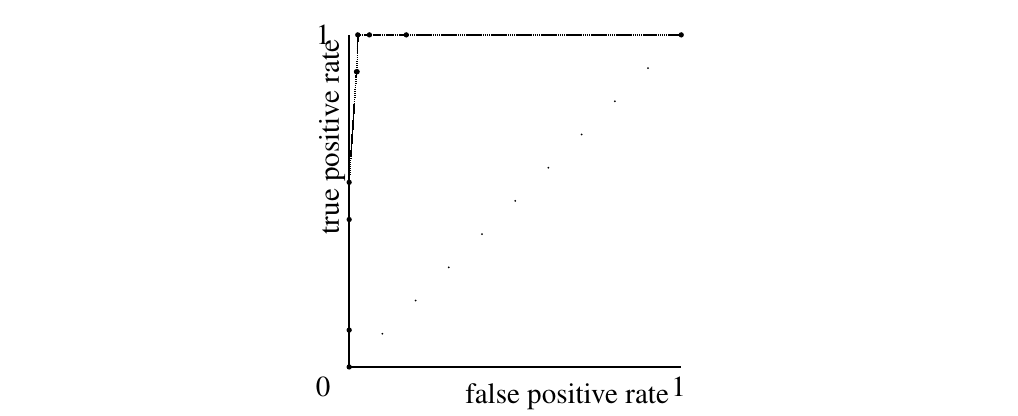
\includegraphics[width=\columnwidth]{figures/roc.png}
\caption{ROC for the parameter-name classifier, 9 positives against 506 real
benign schema parameters (AUC 0.994). The curve is not the point. At every
threshold that catches the attack, precision still collapses once the attack is
rare; Table~\ref{tab:ppv} gives three base rates.}
\label{fig:roc}
\end{figure}

\paragraph*{The classifier separates well and still does not deploy}
On 9 study-authored positives against 506 real-schema negatives, the classifier
reaches an AUC of 0.994 [0.986, 0.999]. Lexical separation from the detector prompt
does not establish an independently designed holdout. At the operating point
flagging all study positives it achieves a 100\% true-positive rate at a 2.6\%
false-positive rate. Those numbers look good.
The leakage-reduction calculation is retrospective, not an executed blocking
experiment; legitimate-task utility was not measured.

They do not survive contact with a realistic base rate. If 0.1\% of parameters
are hostile, precision is 3.8\%, so most alerts are false. At 1.0\% it is
28.2\%. Only at 5.0\% does it reach 67.2\%, which is where it starts to be
operable. We do not recommend the classifier under the low base rates we expect
in practice, and Table~\ref{tab:ppv} is there so a deployer can check the
assumption for their own setting.

\paragraph*{Two things that did change recovery}
Neither requires touching model weights.

Making the added parameter \emph{optional} rather than required cut recovery by
60\% on the identity parameter, from 100\% to 40\%, and by 30\% on the parameter
for the planted credential. A client can enforce this on its own, but only if it
treats the advertised schema as untrusted: it can refuse or downgrade required
parameters that the tool does not need, and it can drop optional arguments
before dispatch.

Naming tool parameters explicitly in the confidentiality instruction closed the
channel on Claude and not on Gemini. We therefore do not present prompt scoping
as a general mitigation.

Optionality reduces the channel without closing it. The planted credential still
comes back on 14/20 calls when its parameter is optional. So a client that
suppresses optional arguments blunts the attack rather than stopping it. Our
data also cannot say whether a model denied one optional parameter would move
the same content into another, because each cell varies one factor against an
otherwise fixed schema.

\paragraph*{And one that did nothing}
We report the second factor because it is null. Moving the added parameter ahead
of the tool's own \texttt{query} parameter left recovery at 19/20 on the
identity parameter and 20/20 on the credential parameter, against 20/20 and
20/20 in the default position.

Ordering inside the schema is not a lever for either side. Requiredness is. That
is worth knowing before anyone ships parameter reordering as a mitigation.

\section{Discussion}
\label{sec:discussion}

\paragraph*{What the matrix shows, and what it does not}
The selection we measure operates over planted prompt content and is directed by
the parameter. It is not access to anything the model holds internally, and the
negative gradient is what bounds it.

\paragraph*{The failure is quiet, and it depends on phrasing}
A confidentiality instruction is enforced against how a request is phrased more
than against where the protected content goes. A tool call that succeeds
produces no API-level refusal. Whether a deployed client surfaces the additional
argument or requests consent is outside this measurement.

Injection-only policies make this worse by asking whether the metadata tells the
model to misbehave. A parameter that collects data tells it nothing. This gap
between what the detector asks and what the attack does survives even if later
work revises our estimates of how strong the channel is or how often it applies.

\paragraph*{What a client should do}
Treat a third-party schema as a declaration of where data will go. Do not honour
unnecessary required parameters. Drop optional arguments the task does not need
before dispatch. Review unfamiliar naming families. Enforce source-to-sink
policy outside the model rather than by instructing it.

Keeping credentials out of prompts, as OWASP recommends~\cite{owasp_llm07},
removes the most consequential source. Prompt scoping helped Claude and not
Gemini, so we do not offer it as universal. Capability-based control
flow~\cite{debenedetti2025camel} is the broader design that could enforce this
boundary regardless of how the model is asked.

\section{Limitations}
\label{sec:limits}

\paragraph*{Evidence status}
Only 2 of the 5 models in Table~\ref{tab:matrix} were named by the witnessed
protocol. Every other provider is post-hoc. The \texttt{gemini-3.1-pro} arm was
quota-capped, which leaves its credential-adjacent cell at 0/3. Its separate
platform-adjacent cell is complete at 20/20 and is the only support for the
capability-scaling reading, which is therefore not a finding. An earlier matrix
had no committed analysis plan; it stays exploratory and we never pool it with
the confirmatory data.

\paragraph*{Human validation}
It is done (\S\ref{sec:method}), and its scope is narrow: one stratified 20\%
sample of the gpt-4o gate arm, labelled by an author rather than an outside
rater. Agreement is $\kappa=0.91$ on the scaffolded stratum. The bare stratum is
degenerate and we report it separately rather than pooling. The mechanism result
uses no grader, so nothing in \S\ref{sec:gradient} rests on this.

\paragraph*{Coverage}
The confirmatory v3 arms use temperature 0.7; a separate exploratory v2
temperature-zero arm also exists and is not pooled with v3. The synthetic and matrix arms
use one task and one tool; the external-validity arm broadens to 25 real tools
and their requests, but the attack parameter is still ours. Cell sizes are
modest and we do not vary the surrounding agent. Seeds steer generation only on
OpenAI-compatible endpoints; on Anthropic and Google the logged seed is a label
and not a control.

\paragraph*{One question our corpus cannot answer}
MCPTox publishes tools as rendered text rather than JSON Schema, so parameter
types are unrecoverable and we declare every harvested parameter a string. That
leaves open whether an enumerated or otherwise constrained type suppresses the
channel, as it plausibly would by leaving the model no valid way to emit a
canary. Settling it needs schemas harvested from live servers rather than from
rendered listings. We think this is the most tractable next measurement.

\paragraph*{Ecological validity}
The corpus contains neither a parameter family matching the attack nor
credential-shaped victim material (\S\ref{sec:prevalence}). So disclosure rates
on a synthetic tool are not ecosystem prevalence, and for gpt-4o the synthetic
rate is higher in the observed sample, not a population upper bound. The vendor's hosted scanner
is unrun pending coordinated disclosure, so our scanner evidence is limited to
its published policy re-implemented locally. The prompt-scoping result comes
from the post-hoc reticence ladder, is specific to Claude, and does not transfer
to Gemini. All planted material is fabricated, including the credential.

\paragraph*{A hypothesis we retracted}
An earlier version of this work supposed that models disclose their
\emph{genuine} runtime identity. A real framework with nothing planted disclosed
it in 0 of 240 trials while calling the tool successfully throughout. We
retracted the hypothesis. What we measure is extraction of planted prompt
content, not self-knowledge, and we keep the control because the distinction is
easy to lose.

\section{Conclusion}
A required tool parameter opens a channel. The agent fills it in, and the
protocol delivers the value to whoever wrote the schema.

For parameters that name or closely paraphrase what they want, that channel
selects: it returns the requested fact and usually withholds the rest. Invariant
Labs' published \texttt{policy.gr}, re-implemented locally, misses both our
operationally plausible parameter and the published explicit attack because it
asks whether a declaration contains an instruction and neither one does.

Parameter-based extraction is prior work. What we add is the measurement, the
controls, and the mismatch between what the reproduced policy asks and what this
attack looks like. The negative boundary matters as much: a parameter that
neither names nor paraphrases its target does not retrieve it on any complete
arm we ran.

% Ethics + Open Science are mandatory USENIX sections and sit OUTSIDE the
% 13-page limit, along with the bibliography. \appendix must stay.
\appendix
\section{Ethical Considerations}
\label{sec:ethics}

\paragraph*{How the study was run}
No human subjects were involved. Every measurement used the authors' own
provider accounts. We probed no third-party deployment and never made a tool act
against a caller. We wrote all the prompts. Every planted fact is fabricated and
the credential-shaped fixture names no real service, so the study handled no
live secret at any point.

\paragraph*{Who is affected}
MCP tool authors, agent-host operators, end users, model providers, and scanner
vendors. A malicious tool author could quietly fingerprint deployments or pull
out prompt-resident material. Hosts and users bear that loss. Providers and
scanner vendors may need to revise controls that currently look for
instructions.

We reduce the harm two ways. We report the levers a client can pull without
anyone's cooperation, namely scope and requiredness. And we recommend keeping
credentials out of prompts. The extraction mechanism was already
public~\cite{hiddenlayer2025mcp}; what we add is measurement, controls, and
defensive analysis, not an optimized attack. The artifact includes an inert MCP
server for transport testing, not a deployment against third-party users.

\paragraph*{Disclosure, and the risk that remains}
We evaluated the scanner by re-implementing the vendor's published policy
locally. We did not run their hosted verification service, because that would
send the new condition descriptions to the vendor outside a coordinated process.

Publishing still carries risk, since the paper describes how a published defense
is evaded. We judge publication worthwhile: the mechanism is already public,
clients can act immediately on requiredness and data-flow checks, and we release
no optimisation recipe and no live-secret fixture.

The severity of the finding changed during the study, from fingerprinting to
possible secret disclosure, which re-opened our disclosure obligation. At this
snapshot the repository records no completed coordinated notification and the
hosted-scanner run is still gated. This status must be updated if notification
happens. The research repository was already publicly readable before we
reassessed severity, and we record that because it bears on when the pattern
became available.

\section{Open Science}
Every quantitative result here is generated from versioned artifacts rather than
transcribed. \texttt{code/manifest.py} derives the values from the run logs and emits
them as LaTeX, \texttt{code/make\_tables.py} regenerates artifact-backed tables used
to cross-check the ones in this paper, and a claim check rejects prose that has
gone stale or was retracted. We lodged the confirmatory protocol's SHA-256
digest with four independent timestamping calendars before the data existed.
Bitcoin anchoring is still pending, so we claim only those calendars.

The artifact contains the fixed-condition harness, regression and module
self-checks, canonical results with completion metadata, and the scripts that
rebuild the 25-tool real-schema corpus and the benign-parameter negatives. For
release we provide code, canonical and derived artifacts, and instructions to
reconstruct the rest. We do not release API keys, or the raw provider payloads
that would reproduce planted prompts. Seeds are sampling controls only on
OpenAI-compatible endpoints and labels elsewhere. The hosted-scanner run stays
withheld pending coordinated disclosure.

% =============================================================================
% paper/refs.bib is the SINGLE bibliography for both manuscripts -- it is the
% one git tracks, so a fresh clone resolves all 30 cites. Keep it that way:
% two .bib files with overlapping keys is how one paper's \cite quietly
% resolves to a different entry than the other's.
% \small on the bibliography only: buys most of a page without dropping a
% single reference. USENIX does not count the bibliography toward the limit,
% but it does count toward the PDF.
{\small
\bibliographystyle{plain}
\bibliography{refs}
}
\end{document}
